\documentclass{beamer}
\usepackage[utf8]{inputenc}
\usepackage{uniinput}
\usepackage[english]{babel}
\usepackage{xstring}
\usepackage{ulem}
\usepackage{boxedminipage} 
\usepackage{xspace} 

\usepackage{tikz}
\usetikzlibrary{chains,fit,shapes}

\usetheme{Madrid}
\usecolortheme{seahorse}
\setbeamertemplate{navigation symbols}{}
\setbeamertemplate{footline}[frame number]
\setbeamertemplate{headline}{%
\leavevmode%
  \hbox{%
    \begin{beamercolorbox}[wd=\paperwidth,ht=2.5ex,dp=1.125ex]{palette quaternary}%
    \insertsectionnavigationhorizontal{\paperwidth}{}{\hskip0pt plus1filll}
    \end{beamercolorbox}%
  }
}

\newcommand{\SO}{\ensuremath{\mathrm{SO}}}
\newcommand{\FO}{\ensuremath{\mathrm{FO}}}
\newcommand{\NP}{{\rm NP}\xspace}
\newcommand{\SAT}{{\rm SAT}\xspace}
\newcommand{\structa}{\ensuremath{\mathfrak{A}}}
\newcommand{\minel}{\ensuremath{\underline{\mathrm{min}}}}
\newcommand{\blankcell}{\ensuremath{T_{\Box}}}
\newcommand{\nonblankcell}{\ensuremath{T_{\blacksquare}}}

\renewcommand{\L}{\mathcal{L}}
\newcommand{\K}{\mathcal{K}}
\newcommand{\A}{\mathcal{A}}
\renewcommand{\P}{\mathcal{P}}

\title{Turing Machines and Finite Models}
\author{Matthias Schlaipfer \and Sebastian Zivota}
\date{February 5, 2015}

\begin{document}

\begin{frame}[plain]
	\titlepage
\end{frame}

%\begin{frame}
%	\frametitle{Outline}
%	\tableofcontents
%\end{frame}

\begin{frame}
  \frametitle{Outlook}
  \begin{itemize}
    \item Connection between finite model theory and complexity theory
    \item By coding Turing machines in various logics
  \end{itemize}
  \vspace{2em} 
  \begin{alertblock}{Important Results}
  \begin{itemize}
    \item Trakhtenbrot's theorem: Finite satisfiability is undecidable
    \item Fagin's theorem: $\exists \SO$ captures $\mathrm{NP}$
  \end{itemize}
  \end{alertblock}
\end{frame}

\section{Background}

\begin{frame}
  \frametitle{Turing Machines}

  \begin{block}{Notation}
    $M = (Q, \Sigma, \Delta, \delta, q_0, Q_a, Q_r)$
    \begin{itemize}
      \item $Q$ \ldots states
      \item $\Sigma$ \ldots input alphabet
      \item $\Delta$ \ldots tape alphabet
      \item $\delta$ \ldots transition function
      \item $q_0$ \ldots initial state
      \item $Q_a$ / $Q_r$ \ldots accepting / rejecting states
    \end{itemize}

  \end{block}

  \begin{center}
  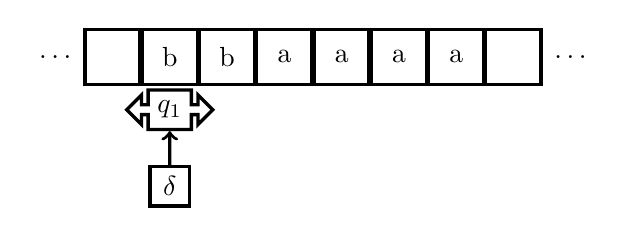
\begin{tikzpicture}
    \tikzstyle{every path}=[very thick]

    \edef\sizetape{0.7cm}
    \tikzstyle{tmtape}=[draw,minimum size=\sizetape]
    \tikzstyle{tmhead}=[arrow box,draw,minimum size=.5cm,arrow box
    arrows={east:.25cm, west:0.25cm}]
    \tikzstyle{tmprog}=[draw,minimum size=.5cm]

    %% Draw TM tape
    \begin{scope}[start chain=1 going right,node distance=-0.15mm]
        \node [on chain=1,tmtape,draw=none] {$\ldots$};
        \node [on chain=1,tmtape] {};
        \node [on chain=1,tmtape] (input) {b};
        \node [on chain=1,tmtape] {b};
        \node [on chain=1,tmtape] {a};
        \node [on chain=1,tmtape] {a};
        \node [on chain=1,tmtape] {a};
        \node [on chain=1,tmtape] {a};
        \node [on chain=1,tmtape] {};
        \node [on chain=1,tmtape,draw=none] {$\ldots$};
    \end{scope}

    %% Draw TM head below (input) tape cell
    \node [tmhead,yshift=-.3cm] at (input.south) (head) {$q_1$};
    \node [tmprog,yshift=-.7cm] at (head.south) (prog) {$\delta$};
    \draw [->] (prog) to (head);

    \end{tikzpicture}
    \nocite{tm_figure}
    \end{center}
  
\end{frame}

\begin{frame}
  \frametitle{Computability Theory}

  A formal language $\mathfrak{L}$ is \ldots
  \begin{itemize}
    \item \textbf{decidable:} There is a TM that decides whether a given string
    is in $\mathfrak{L}$ or not.
    \item \textbf{semidecidable:} There is a TM that answers correctly for a
    string in $\mathfrak{L}$, but may not give an answer otherwise.
    \item \textbf{undecidable:} There is no TM to decide whether a given string
    is in $\mathfrak{L}$ or not.
  \end{itemize}

  
\end{frame}

\begin{frame}
  \frametitle{Some Results on TM}

  \begin{itemize}
    \item The \textbf{halting problem} is undecidable.
    \item The \textbf{blank tape halting problem} is undecidable.
      \begin{center}
        \begin{boxedminipage}{.5\textwidth}
          \begin{tabbing}
            \quad\=\quad\=\quad\=\kill\\
                {\tt halts?}$(M,x)$\\
                \>{\tt if} $\mathsf{encode}(\mathsf{sim}(M, x)) \in \mathbf{BTHP}$\\
                \>\>yes\\
                \>{\tt else}\\
                \>\>no\\
          \end{tabbing}
        \end{boxedminipage}
      \end{center}
  \end{itemize}
  
\end{frame}

\begin{frame}
  \frametitle{Some Results on FOL}

  \begin{itemize}
    \item Completeness: a sentence $\phi$ is valid iff it is provable
    \item Proofs can be enumerated $\longrightarrow$ valid $\FO$ sentences
    recursively enumerable
  \end{itemize}

  \begin{definition}[Validity]
    All structures $\structa$, finite or infinite, are models of $\phi$.
    ($\structa \models \phi$)
  \end{definition}
  
\end{frame}

\section{Trakhtenbrot's Theorem}

\begin{frame}
  \frametitle{Trakhtenbrot's Theorem and Failure of Completeness}

  \begin{definition}[Finite satisfiability]
    Given a vocabulary $\sigma$, a sentence $\phi$ in that vocabulary is called
    finitely satisfiable if there is a finite structure $\structa \in
    \mathrm{STRUCT}[\sigma]$ such that $\structa \models \phi$.
  \end{definition}
  
  \pause

  \begin{theorem}[Trakhtenbrot]
    For every relational vocabulary $\sigma$ with at least one binary relation
    symbol, it is undecidable whether a sentence $\phi$ of vocabulary
    $\sigma$ is finitely satisfiable.
  \end{theorem}

\end{frame}

\begin{frame}
  \frametitle{Proof Idea}

  \begin{itemize}
    \item Code Turing machines in $\FO$
    \item For every TM $M$, construct a sentence $\phi_M$ of vocabulary $\sigma$
    such that $\phi_M$ is finitely satisfiable iff $M$ halts on the empty input.
  \end{itemize}

\end{frame}

\begin{frame}
  \frametitle{Definitions}

  \begin{itemize}
    \item $\sigma = \{<, \minel, \blankcell(\cdot, \cdot),
    \nonblankcell(\cdot,\cdot), (H_q(\cdot, \cdot))_{q \in Q}\}$\\
    \item $<$ is a linear order and $\minel$ is its minimal element (time,
    positions)
    \item Tape predicates $\blankcell(p,t), \nonblankcell(p,t)$
    \item Head predicates $H_q(p,t)$
  \end{itemize}
  
\end{frame}

\begin{frame}
  \frametitle{Definitions}

  For example at time $t$:
  \begin{center}
  \begin{tikzpicture}
    \tikzstyle{every path}=[very thick]

    \edef\sizetape{0.7cm}
    \tikzstyle{tmtape}=[draw,minimum size=\sizetape]
    \tikzstyle{tmhead}=[arrow box,draw,minimum size=.5cm,arrow box
    arrows={east:.25cm, west:0.25cm}]
    \tikzstyle{tmprog}=[draw,minimum size=.5cm]

    %% Draw TM tape
    \begin{scope}[start chain=1 going right,node distance=-0.15mm]
        \node [on chain=1,label={[label distance=2ex,text depth=5ex,rotate=90]right:$\minel$},tmtape] {$\Box$};
        \node [on chain=1,label={[label distance=2ex,text depth=5ex,rotate=90]right:$\minel+1$},tmtape] (input) {$\blacksquare$};
        \node [on chain=1,label={[label distance=2ex,text depth=5ex,rotate=90]right:$\minel+2$},tmtape] {$\blacksquare$};
        \node [on chain=1,label={[label distance=2ex,text depth=5ex,rotate=90]right:$\minel+3$},tmtape] (blankcell) {$\Box$};
        \node [on chain=1,label={[label distance=2ex,text depth=5ex,rotate=90]right:$\minel+4$},tmtape] {$\Box$};
        \node [on chain=1,label={[label distance=2ex,text depth=5ex,rotate=90]right:$\minel+5$},tmtape] {$\Box$};
        \node [on chain=1,label={[label distance=2ex,text depth=5ex,rotate=90]right:$\minel+6$},tmtape] {$\Box$};
        \node [on chain=1,label={[label distance=2ex,text depth=5ex,rotate=90]right:$\minel+7$},tmtape] {$\Box$};
        \node [on chain=1,tmtape,draw=none] {$\ldots$};
    \end{scope}

    %% Draw TM head below (input) tape cell
    \node [tmhead,yshift=-.3cm] at (input.south) (head) {$q_9$};
    %\node [tmprog,yshift=-1.7cm] at (head.south) (prog) {$\delta$};
    %\draw [->] (prog) to (head);

    \node at (4,-1) {$\blankcell(\minel+3, t)$} edge[->,bend left=15] (blankcell.south);
    \node at (3,-2) {$H_{q_9}(\minel+1, t)$} edge[->,bend left=25] (head.south);

    \end{tikzpicture}
    \nocite{tm_figure}
    \end{center}
  
\end{frame}

\begin{frame}
  \frametitle{Encoding}

  \centering
  \begin{enumerate}
    \only<1->{\item $<$ is a linear order and $\minel$ is its minimal element}
    \only<2->{\item Initially the tape is blank}
      \only<2>{\begin{align*}
        H_{q_0}(\minel, \minel) \wedge \forall p \; \blankcell(p, \minel)
      \end{align*}}
    \only<3->{\item Either a cell is blank or not}
      \only<3>{\begin{align*}
        \forall p \forall t \;
        \left(\blankcell(p, t)
        \Leftrightarrow \neg \nonblankcell(p, t)\right)
      \end{align*}}
    \only<4->{\item Machine is in one state at a time}
      \only<4>{\begin{align*}
        \forall t \exists !p &\left( \bigvee_{q \in Q} H_q(p,t) \right)
        \wedge \\ \neg \exists p \exists t &\left( \bigvee_{q, q' \in Q, q \neq q'}
        H_q(p, t) \wedge H_{q'}(p,t) \right)
      \end{align*}}
    \only<5->{\item Machine respects the transition relation}\only<5>{ e.g.
    $\delta(q, \Box) = (q', \blacksquare, \ell)$}
      \only<5>{\small \begin{align*}
        \forall p \forall t \;
        \left(
          \begin{array}{cc}
                   & p \neq \minel\\
            \wedge & \blankcell(p, t)\\
            \wedge & H_q(p,t)
          \end{array}
        \right)
          \Rightarrow
        \left(
          \begin{array}{cl}
                   & \nonblankcell(p, t+1)\\
            \wedge & H_{q'}(p-1, t+1)\\
            \wedge &
              \begin{array}[x]{@{}l@{}} 
            \forall p' \; \left(p \neq p' \Rightarrow \right. \\ \left. \left( \bigwedge_{i =
            \Box,\blacksquare} T_i(p',t+1) \Leftrightarrow
            T_i(p',t)\right)\right)
              \end{array}
          \end{array}
        \right)
      \end{align*}}
    \only<6->{\item Finally, the machine halts}
      \only<6>{\begin{align*}
        \exists p \exists t \; \bigvee_{q \in Q_a \cup Q_r} H_q(p,t)
      \end{align*}}
  \end{enumerate}
  
\end{frame}

\begin{frame}
  \frametitle{Proof}

  \begin{theorem}[Trakhtenbrot]
    For every relational vocabulary $\sigma$ with at least one binary relation
    symbol, it is undecidable whether a sentence $\phi$ of vocabulary
    $\sigma$ is finitely satisfiable.
  \end{theorem}
  
  \begin{alertblock}{Proof}

  \begin{itemize}
    \item A finite model of $\phi_M$ represents a computation of $M$ starting
    from blank tape to a halting state
    \item The set of all configurations of the halting computations of $M$ is a
    finite model of $\phi_M$
  \end{itemize}

  $M$ halts on the empty input iff $\phi_M$ has a finite model. Since
  \textbf{BTHP} is undecidable, so is finite satisfiability for $\phi_M$.
  \end{alertblock}
  
\end{frame}

\begin{frame}
  \frametitle{Corollaries}

  \begin{corollary}[Failure of completeness in the finite]
    For any vocabulary containing at least one binary relation symbol, the set
    of finitely valid sentences is not recursively enumerable.
  \end{corollary}

  \begin{corollary}[No analog to Löwenheim-Skolem for finite models]
    There is no recursive function $f$ such that if $\phi$ has a finite model,
    then it has a model of size at most $f(\phi)$.
  \end{corollary}
  
\end{frame}

\section{Fagin's Theorem}

\begin{frame}

\huge
\centering Fagin's Theorem
  
\end{frame}

\begin{frame}
  %\frametitle{title}

	Goal: Machine-independent characterization of complexity classes
	\begin{definition}<2->
		Let $\mathcal{K}$ be a complexity class and $\mathcal{L}$ a logic. We say that $\L$ captures $\K$ if the following holds:
		\begin{enumerate}
			\item For every sentence $Φ$ of $\L$ and every finite structure $\A$, it is decidable in $\K$ whether $\A \vDash Φ$;
			\item For every property $\P$ of finite structures decidable in $\K$ there is a sentence $Φ$ of $\L$ such that $\A$ has property $\P$ iff $\A \vDash Φ$.
		\end{enumerate}
	\end{definition}
	
	\medskip
	
	\uncover<3->{Briefly: We say that $\L$ captures $\K$ if the properties that can be decided in $\K$ are exactly those that can be defined in $\L$.}
	
	\medskip
	
	\uncover<4->{Application: Show that complexity classes are different by showing that their capturing logics are different.}
\end{frame}

\begin{frame}
\frametitle{Fagin's Theorem}
Reminder: $\exists SO$ is second order predicate logic with only existential second order quantifiers.
  \begin{theorem}[Fagin]<2->
    $∃SO$ captures $NP$.
  \end{theorem}
  \uncover<3->{That is: the $NP$-decidable properties of finite structures are exactly those that $∃SO$ can express.}
  
  \medskip
  
  \uncover<4->{First machine-independent characterization of a complexity class (1974).}
 \begin{corollary}<5->
  $\forall SO$ captures $coNP$.
 \end{corollary}
  \uncover<6->{Application to the $P = NP$ problem:
  \begin{equation*}
   \forall SO \neq \exists SO \Rightarrow coNP \neq NP \Rightarrow P \neq NP
  \end{equation*}}
\end{frame}

\begin{frame}
  \frametitle{Encoding Structures}
  \begin{tabular}{rcl}
    $enc(\A)$ &…& encoding of structure $\A$ as a string of bits.\\
    $\|\A\|$ &…& length of $enc(\A)$. Polynomial in $|A|$.
  \end{tabular}
 
  \medskip
 
  \begin{block}{Example}<2->
  $\A = (A, E)$ with $A = \{0,…,n-1\}$ and $E$ binary.
	
  \medskip
	
  \uncover<3->{$enc(\A) = 0^n1\cdot s$, with $s$ a string of length $n^2$ that encodes $E$:}
  
  \uncover<4->{\begin{align*}
    s_{in+j} &= \begin{cases} 1 &\text{if } i {E} j,\\ 0 &\text{otherwise.} \end{cases}\\
    s &= \underbrace{s_0…s_{n-1}}_{\text{edges from $0$}}\underbrace{s_n…s_{2n-1}}_{\text{edges from $1$}}…\underbrace{s_{n(n-1)}…s_{n^2-1}}_{\text{edges from $n-1$}}
  \end{align*}}
  \end{block}
\end{frame}


\begin{frame}
 \frametitle{Proof of Fagin's Theorem}
 Easy direction: Let $Φ$ be a sentence of $\exists SO$ and $\A$ a structure. Suppose $Φ = \exists S_1 … \exists S_n Ψ$ with $Ψ$ FO. Checking whether $\A \vDash Φ$ can be done by guessing $S_1,…,S_n$ and then checking $\A \vDash Ψ(S_1,…,S_n)$. The latter part is polynomial in $\|\A\|$.
 
 \medskip
 
 \uncover<2->{Hard direction: Similar to proof of Trakhtenbrot's theorem, but a bit more involved.}
 \begin{itemize}
 	\item<3-> Given: ND Turing machine $M$ that takes encodings of structures as input and tests whether property $\P$ holds.
 	\item<4-> If $n$ is the size of the structure, assume that $M$ runs in time $n^k$ for some $k$ and visits the entire input.
 	\item<5-> Can describe both time and space on tape as $k$-tuples of elements of the model.
 \end{itemize}
\end{frame}

\begin{frame}
	\frametitle{Hard direction, ctd.}
	We seek to construct a sentence
	\begin{equation*}
	Φ = ∃L ∃T_0 ∃T_1 ∃T_{\_} ∃H_{q_0} … ∃H_{q_{m-1}} Ψ,
	\end{equation*}
	such that $\A \vDash Φ$ iff $M$ terminates in an accepting state on $enc(\A)$.
	
	\medskip
	
	\uncover<2->{$L$ is binary and the other predicates are $2k$-ary.}
	
	\medskip
	
	\uncover<3->{Intended interpretation of the predicates:}
	\begin{itemize}
	\item<3-> $L$ is a linear order. Define lexicographic order $<_k$ based on $L$.
	\item<4-> $T_{*}(\bar{p}, \bar{t})$ … tape contains $*$ at position $\bar{p}$ and time $\bar{t}$ for $* ∈ \{0, 1, \_\}$.
	\item<5-> $H_{q_i}(\bar{p},\bar{t})$ … at time $\bar{t}$, the machine is in state $q_{i}$ and the head is in position $\bar{p}$.
	\end{itemize}
\end{frame}

\begin{frame}
	\frametitle{Construction of $Ψ$}
	$Ψ$ is a conjunction of several formulas:
	\begin{itemize}
		\item<2-> $L$ is a linear order.
		\item<3-> Tape and state are well-defined and $M$ eventually arrives in an accepting state. Exactly as in the proof of Trakhtenbrot.
		\item<4-> Sentences describing the transition function: For $a ∈ Δ, q ∈ Q$,
		\begin{equation*}
		\bigvee_{(q',a',mv) ∈ δ(q,a)} α_{(q,a,q',a',mv)},
		\end{equation*}
		where $α_{(q,a,q',a',mv)}$ is as in the previous proof.
		\item<5-> A formula describing the initial state of the tape (i.e. $enc(\A)$):
		\begin{equation*}
		∀\bar{p}∀\bar{t}\left(¬∃\bar{u} (\bar{u} <_k \bar{t}) → \left[
		\begin{array}{rcl}
		ι(\bar{p})&\leftrightarrow&T_1(\bar{p},\bar{t})\\
		∧\ ξ(\bar{p})&\leftrightarrow&T_{\_}(\bar{p},\bar{t})
		\end{array}		
		\right]\right)
		\end{equation*}
	\end{itemize}
\end{frame}

\begin{frame}
	\frametitle{Construction of $ι(\bar{p})$ and $ξ(\bar{p})$}
	\begin{block}{Initial state of $M$}
	\begin{equation*}
		∀\bar{p}∀\bar{t}\left(¬∃\bar{u} (\bar{u} <_k \bar{t}) → \left[
		\begin{array}{rcl}
		ι(\bar{p})&\leftrightarrow&T_1(\bar{p},\bar{t})\\
		∧\ ξ(\bar{p})&\leftrightarrow&T_{\_}(\bar{p},\bar{t})
		\end{array}		
	\right]\right)
	\end{equation*}
	\medskip
	\begin{tabular}{rcl}
	$ι(\bar{p})$ &…& $enc(\A)$ contains $1$ at position $\bar{p}$\\
	$ξ(\bar{p})$ &…& $\bar{p}$ is outside of $enc(\A)$, i.e. $\bar{p} >_k \|\A\|$
	\end{tabular}
	\end{block}
	\uncover<2->{Recall $enc(\A)$ for a graph:
	\begin{align*}
	 enc(\A) &= 0^n1s_0…s_{n^2-1},\\
	 s_{in+j} &= \begin{cases} 1 &\text{if } i {E} j,\\ 0 &\text{otherwise.}\end{cases}
	\end{align*}}

	\uncover<3->{Suppose $k = 3$. Then a tuple $\bar{p} = (p_1,p_2,p_3)$ represents the position $p_1 n^2 + p_2 n + p_3$.}
\end{frame}

\begin{frame}
 \frametitle{Construction of $ι(\bar{p})$ and $ξ(\bar{p})$, ctd.}
 \begin{equation*}
  enc(\A) = 0^n1s_0…s_{n^2-1}
 \end{equation*}

 Construct $ι$ and $ξ$ by case distinction:
 \begin{itemize}
  \item<2-> Positions $0,…,n-1$ are certainly $0$.
  \item<3-> Position $n$ is certainly $1$.
  \item<4-> Treat positions $n+1$ to $n^2 + n$ according to $E$.
  \item<5-> All positions from $n^2 + n + 1$ onward must be blank.
 \end{itemize}
%	\begin{align*}
%	p_1 > 1 &\Rightarrow ι(\bar{p}) = \bot\\
%	p_1 = p_2 = 0 &\Rightarrow ι(\bar{p}) = \bot\\
%	p_1 = 0, p_2,p_3 \neq 0 &\Rightarrow ι(\bar{p}) = E(p_2-1, p_3-1)\\
%	p_1 = p_3 = 0, p_2 \neq 0 &\Rightarrow ι(\bar{p}) = E(p_2-2, n-1)
%	\end{align*}

  \vspace*{-0.5cm}
  
  \begin{align*}
  \uncover<3->{ι(\bar{p}) &= \left[p_1 = 0 ∧ p_2 = 1 ∧ p_3 = 0\right]\\}
  \uncover<4->{&∨\ \left[\left(\begin{array}{rcl}
  p_1 &=& 0 \\
  ∧\ p_2 &>& 0
  \end{array}\right) ∧ \left(\begin{array}{rclcl}
  p_3 &\neq& 0 &∧& E(p_2-1, p_3-1)\\
  ∨\ p_3 &=& 0 &∧& E(p_2-2, n-1)
  \end{array}\right)\right]\\}
  \uncover<4->{&∨\ \left[p_1 = 1 ∧ … \right]\\}
  \uncover<5->{ξ(\bar{p}) &= (p_1 > 1) ∨ \left(p_1 = 1 ∧ p_2 > 1\right) ∨ \left(p_1 =1 ∧ p_2 = 1 ∧ p_3 > 0\right)}
  \end{align*}
  %\uncover<3->{Here, $x = 0$ means $¬∃y (y < x)$, etc.}
  \uncover<6->{This concludes the proof of Fagin's theorem. \qed}
\end{frame}

\begin{frame}
  \frametitle{Corollaries}

  \begin{corollary}[Cook]
    \SAT is \NP-complete
  \end{corollary}

  \only<1>{
  \begin{alertblock}{Proof}
    $\mathcal{P} \in \NP$
    \begin{itemize}
      \item $\phi \equiv \exists S_1, \ldots, \exists S_n \; \varphi$, such that
      $\structa$ is in $\mathcal{P}$ iff $\structa \models \phi$ (Fagin)
      \item $X = \{S_i(\vec{a}) \; | \; i = 1, \ldots, n, \vec{a} \in
      A^{\text{arity}(S_i)}\}$
      \item $\structa \models \phi$ iff $\alpha_{\phi}^{\structa}$ is
      satisfiable
      \item $\alpha_{\varphi}^{\structa}$ is obtained from $\varphi$
        \begin{itemize}
          \item replace $\exists x \, \psi(x, \cdot)$ by $\bigvee_{a \in A}
          \psi(a, \cdot)$
          \item replace $\forall x \, \psi(x, \cdot)$ by $\bigwedge_{a \in A}
          \psi(a, \cdot)$
          \item replace $R(\vec{a})$, for $R \in \sigma$ by its truth value in
          $\structa$
        \end{itemize}
      \item $\structa \models \phi$ iff $\alpha_{\varphi}^{\structa}$ is
      satisfiable. $\alpha_{\varphi}^{\structa}$ can be constructed by
      deterministic logarithmic space machine
    \end{itemize}
  \end{alertblock}
  }

  \only<2>{
  \begin{corollary}
    $\SO$ captures the polynomial hierarchy
  \end{corollary}
  }
\end{frame}



\section{}
\bibliography{presentation}
\bibliographystyle{plain}
\end{document}
